\chapter{\uppercase{Results And Discussion}}\label{Ch:Results}

In this chapter we will explain the results of all the 192 experiments on our dataset. We measure the results using the overall accuracy Then we measure the performance accuracy of the model per class (meter). We will start by present the results for every combinations and then discuss our findings related to the topic.

\section{Results}

As we explained, In Chapter~\ref{Ch:Model_Training} we have a set of combinations we need to explore it. So, most of our results will combine a combination and show the results of these combinations. Let's explore it as below,
\begin{enumerate}
\item  We have three data representation \textbf{\textit{Binary, One-hot, and Two-Hot}} we will represent it as \textbf{\textit{BinE, 1D, 0T}} respectively.
\item We have two types of model loss functions \textbf{\textit{Weighting loss and no Weighting loss}} we will represent it as \textbf{\textit{(1 and 0)}} respectively.
\item The Number of layers is represented as \textbf{\textit{nL}}, for example, 7 layers are 7L.
  \item The Number of cell units is represented as \textbf{\textit{nU}}, for example, 82 unit is 82U.
  \end{enumerate}

  So, If we need to explain a set of combination we can write (4L, 82U, 0) which means 4 layers, 82 units, and no weighted loss function. Also, we will provide many figures every figure will explain specific result perspective.
  
\subsection{Overall Accuracy}

% \textbf{$F_1$ (also F-score or F-measure)} is a measure of a test's accuracy. It considers both the precision $p$ and the recall $r$ of the test to compute the score: $p$ is the number of correct positive results divided by the number of all positive results returned by the classifier, and $r$ is the number of correct positive results divided by the number of all relevant samples (all samples that should have been identified as positive).\\ The F1 score is the harmonic average of the precision and recall, where an F1 score reaches its best value at 1 (perfect precision and recall) and worst at 0~\cite{Wiki_f1_score}.

We present the overall accuracy Score in Figure~\ref{Fig:ArabicModelsResults} of the 16 neural networks configurations and at each of the 12 data representations (y- and x-axis respectively). The x-axis is divided into 4 strips corresponding to the 4 combinations of trimming and diacritic parameters. Then, each strip includes the 3 different encoding values. Each point on the figure represents the overall accuracy score of one of the 192 experiments; (some values are too small, and hence omitted from the figure). To explain the figure, we take as an example the most-left vertical list of points that represent the 16 experiments of the full (no trimming), diacritics, and binary encoding dataset representation. For each rug plot, the highest (Bi)LSTM accuracies are labeled differently as circle and square respectively; and the network configuration of both of them is listed at the top of the rug plot.

To explain the figure, we take as an example the most-left vertical rug plot, which corresponds to (0T, 1D, BinE) data representation. The accuracies of the best (Bi)LSTM are 0.9025 and 0.7978 respectively. The configuration of the former is (7L, 82U, 0W). Among all the 192 experiments, the highest accuracy is 0.9638 and is possessed by (4L, 82U, 0W) network configuration on (1T, 0D, BinE) data representation.

%The best network out of the 16 configurations is listed at the top: 7 layers, size of 82, and no loss weighting (7L, 82U, 0W). This network possess 90.25 F1 score by the Bi-LSTM cell (indicated by the large circle).

%The best LSTM model is indicated by the square point, and possess 79.77 F1 score. Among all the 192 experiments, the highest F1 score is 96.38 and is possessed by a network configuration of (4L, 82U, 0) on (1T, 0D, BinE).

\subsubsection{Data Representation Effects}

In this section we will explain the effect of the 12 data representation technique we explained it previous.

\begin{enumerate}
\item \textbf{Trimming Effect:} The effect of trimming (remove the small classes from the training cycle) can be observed if we fix the other two parameters, diacritic and encoding. The score with trimming is consistently higher than that with no trimming. E.g., by looking at the two unshaded strips, the score at (1T, 0D, TwoE) is 0.9629, while that at (0T, 0D, TwoE) is 0.9411. The only exception, with a very little difference, is (1T, 1D, BinE) vs. (0T, 1D, BinE). We need to highlight that is logic to have this effect as the training will have fewer classes with a huge amount of data for these classes.
\item \textbf{Diacritics Effect}
  \begin{itemize}
  \item \textit{Without Trimming:} The effect of diacritics is obvious only with no trimming (the two left strips of the figure), where, for each encoding, the accuracy score is higher for diacritics than no diacritics.
    \item \textit{With Trimming:} The diacritics don't have except for the \textit{one-hot} encoding but other encoding doesn't have an effect on the model performance. This result is inconsistent with what is anticipated from the effect of diacritics. We think that this result is an artifact due to the small number of network configurations.

    \end{itemize} 
\item \textbf{Encoding Effect:} The effect of encoding is clear; by looking at each individual strip, \textit{overall accuracy score is consistently highest for two-hot then one-hot then binary—the} only exception is (1T, 0D, BinE) that performs better than the other two encoding. It seems that two-hot encoding makes it easier for networks to capture the patterns in data. However; we anticipate that there is a particular network architecture for each encoding that can capture the same pattern with yielding the same score.
  \end{enumerate}


  
\begin{figure}[!t]
 \input{./Figures/Ch_7_Results/Fig_overall_Score.tex}
 \caption{Overall accuracy of the 192 experiments plotted as 2 vertical rug plots (for the 12 different data representations: $\left\{\mathit{Trimming},\ \mathit{No Trimming} \right\} \times \left\{\mathit{Diacritics},\ \mathit{No Diacritics} \right\} \times \left\{\mathit{OneE},\ \mathit{BinE},\ \mathit{TwoE}\right\}$), each represents 16 exp. (for the 16 different network configurations: $\left\{7L,\ 4L\right\} \times \left\{82U,\ 50U\right\} \times \left\{0W, 1W\right\} \times \left\{LSTM,\ BiLSTM\right\}$). For each rug plot the best model of each of the four cell types ---(Bi)LSTM labeled differently. Consistently, BiLSTM  was the winner, and its network configuration parameters are listed at the top of each rug plot.}~\label{Fig:ArabicModelsResults}
\end{figure}


  
\subsubsection{Network Configurations Effects} 

This section is to comment on the effect of the network configurations parameters.
\begin{itemize}
\item \textbf{Cell Type}: It is clear that BI-LSTM  (large circle) is the highest accuracy score for each data representation. It is always higher than the highest score of the LSTM model (large square). This is what we expected the more complex architecture, the more results we can achieve. But we need to mention that the BI-LSTM is slower than LSTM in overall running time for all experiments, and it also consumes much more resources than LSTM cell.
\item \textbf{Layers Number:} As we explained in Section~\ref{Sec:Deep_Learning_Background} The idea behind the deep neural network come from the multi-layers which make the network learn more details. So, the more complex network (more layer) the more results we can achieve. So, in our experiments, we can show that 7 layers achieved the highest scores more than the 4 layers. There is an exception for the trimming data without diacritics in (1T, 0D, BinE) and (1T, 0D, TwoE). The straightforward interpretation for that is the reduction in dataset size occurred by trimming and no diacritics, which required a less complex network. So, if we reduced the complexity of our problem the number of layers will not be effective.

\item \textbf{Cell Units and Weighting Loss:} We can't figure out a consistent effect based on the number of cell units or the weighting loss. But we need to mention that the highest results achieved were using both the highest cell units 82 and the weighted loss.
  \end{itemize}



\subsection{Per-Class (Meter) Accuracy}

In this section, we will explore the accuracy of each class. This is regarding how our model can detect every class separately. It similar the previous accuracy but per-class calculation. It is also useful to check it as it will show us how the model able to understand every class and what is the classes which our model not able to classify it. 

Similar in the previous section, We have four combinations of \textit{trimming and diacritic} we will investigate which models achieved the best results. We will take the best four models (the first three of them is the two-hot encoding, and the fourth is the binary encoding) from Figure~\ref{Fig:ArabicModelsResults} which is the overall accuracy and show the results of the per class accuracy for each one.

In Figure~\ref{Fig:Results_Per_Class} we have the previous four models display the per-class accuracy. We ordered The class names based on their data size per class. It explained previously in Figure~\ref{Fig:Data_Size_Distribution} with the same order. If we compare the results for the four models accuracy scores were around 95\% in Figure~\ref{Fig:ArabicModelsResults} and the per-class accuracy, we will find only 6 classes (which have around 80\% of the total datasets) are around this value. But there are significant drops for some classes which make the figures line has dropped in the results.

Figure~\ref{Fig:Results_Per_Class} shows the relation between the model accuracy results per-class and the dataset size per class; However, This trend was expected to be fixed from the weighted loss which has an inconsistent effect of the weighting loss for all the models. This inconsistent effect shows we need to have a new design for has an function which can solve this trending issue. The overall accuracy can be increased after trimming but there will be a gap between the accuracy per class the size of the data per class as the dataset is not balanced. Moreover, We can repeat this experiment again with enforcing all classes to have an equal size so, we can show the accuracy without in data unbalance issue. We will elaborate more in Section~\ref{Sec:Discussion}.



\begin{figure}[!t]
 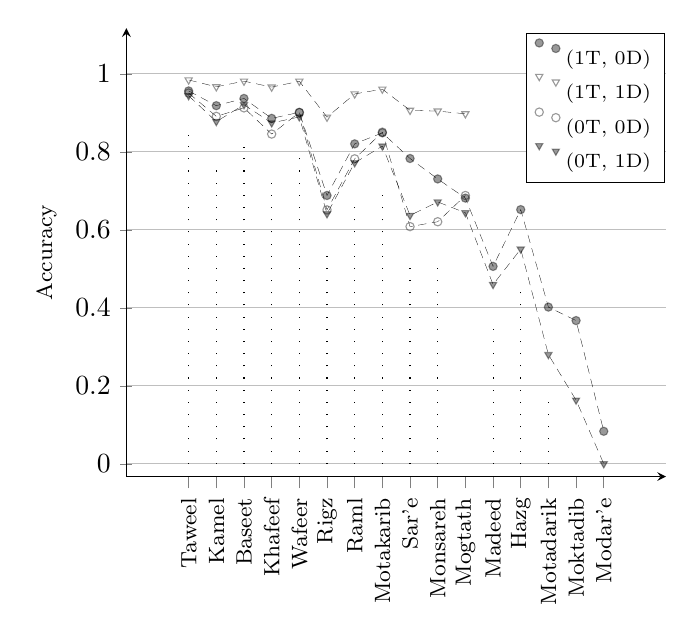
\begin{tikzpicture}[scale=1]
  \begin{axis}[
    axis x line = bottom,
    axis y line = left,
    ymajorgrids = true,
    ybar,
    enlargelimits=0.15,
    legend style={at={(0.87,0.99)},
      anchor=north,legend columns=1},
    ylabel={Accuracy},
    ylabel style = {font=\footnotesize},
    symbolic x coords={Taweel, Kamel, Baseet, Khafeef, Wafeer, Rigz, Raml, Motakarib, Sar'e, Monsareh, Mogtath, Madeed, Hazg, Motadarik, Moktadib, Modar'e},
    xtick=data,
    xticklabel style = {font=\footnotesize},
    nodes near coords align={vertical},
    x tick label style={rotate=90, anchor=east},
    bar width=2pt,
    ymin=0.1,
    ]


	
	% full diacritic (Full Circle)
	% replaced
	% Exp_3_full_data_matrix_with_tashkeel_8bitsEncoding_Bidirectional_LSTM_3_82_0
	% (0T, 1D)
	\addplot[mark=*, thin, only marks, mark size=1.5pt, point
	meta=explicit symbolic, opacity=0.4]
	coordinates {
		(Wafeer,    0.9014024346835623 )       
		(Monsareh,  0.7305790960451978 )       
		(Madeed,    0.5062814070351759 )  
		(Mogtath,   0.6814562002275313 )       
		(Motakarib, 0.8488725411802335 )       
		(Kamel,     0.9185383195083638 )       
		(Taweel,    0.9563337122522612 )       
		(Sar'e,     0.7830334190231363 )       
		(Raml,      0.8205778003041054 )       
		(Rigz,      0.6881982360352793 )       
		(Khafeef,   0.8859834647183235 )       
		(Baseet,    0.9370664229634861 ) 
		(Moktadib,  0.3673469387755102 ) 
		(Hazg,      0.6519480519480519 )
		(Modar'e,   0.08333333333333333)
		(Motadarik, 0.40190476190476193) 
	};


    % trimmed no-diacritic (Empty Triangle)
    \addplot[mark=triangle, every mark/.append style={rotate=180},
    thin, only marks, mark size=1.5pt, point meta=explicit symbolic, opacity=0.4]
    coordinates {
      % replaced
      % Exp_3_eliminated_data_matrix_without_tashkeel_8bitsEncoding_Bidirectional_LSTM_3_82_0
      % (1T, 0D)
      (Wafeer,    0.9811213222198475)       
      (Monsareh,  0.9045746962115797)       
      (Mogtath,   0.897708216880939 )       
      (Motakarib, 0.9609120521172638)       
      (Kamel,     0.966898378020523 )       
      (Taweel,    0.9844991757498216)       
      (Sar'e,     0.9066397034041119)       
      (Raml,      0.9485771342985522)       
      (Rigz,      0.8889925373134329)       
      (Khafeef,   0.9661488673139158)       
      (Baseet,    0.9814341393906374) 
      % Damn Trick; the first \addplot must have all the x ticks; otherwise
      % the following 4 ticks will not appear on the x-axis.
      %(Madeed,     0)  
      %(Hazg,       0) 
      %(Motadarik,  0) 
      %(Moktadib,   0) 
      %(Modar'e,    0)
    };

    % trimmed diacritic (Empty Circle)
    % replaced
    % Exp_3_eliminated_data_matrix_with_tashkeel_8bitsEncoding_Bidirectional_LSTM_3_82_0 
    % (1T, 1D)
    \addplot[mark=o, thin, only marks, mark size=1.5pt, point
    meta=explicit symbolic, opacity=0.4]
    coordinates{
      (Wafeer,     0.9009759920210871)       
      (Monsareh,   0.6208005718370264)       
      (Mogtath,    0.6880939072107323)       
      (Motakarib,  0.8506281991624011)       
      (Kamel,      0.8910956636875207)       
      (Taweel,     0.9508402430922914)       
      (Sar'e,      0.6083586113919784)       
      (Raml,       0.7822016974538193)       
      (Rigz,       0.6512042062415196)       
      (Khafeef,    0.8456957928802589)       
      (Baseet,     0.9128703742508696) 
    };


    % full no-diacritic (Full Triangle)
    % replaced
    % Exp_3_full_data_matrix_without_tashkeel_8bitsEncoding_Bidirectional_LSTM_3_82_0
    % (0T, 0D)
    \addplot[mark=triangle*, every mark/.append style={rotate=180},
    thin, only marks, mark size=1.5pt, point meta=explicit symbolic, opacity=0.4]
    coordinates {
      (Wafeer,    0.889584964761159  )       
      (Monsareh,  0.6716101694915254 )       
      (Madeed,    0.45979899497487436)  
      (Mogtath,   0.6439135381114903 )       
      (Motakarib, 0.8148088917319687 )       
      (Kamel,     0.8776972469479428 )       
      (Taweel,    0.9439529481540059 )       
      (Sar'e,     0.6370179948586119 )       
      (Raml,      0.7719209325899645 )       
      (Rigz,      0.64107517849643   )       
      (Khafeef,   0.8741908607319105 )       
      (Baseet,    0.9208657001620072 ) 
      (Moktadib,  0.16326530612244897) 
      (Hazg,      0.5506493506493506 )
      (Modar'e,   0.0                )
      (Motadarik, 0.28               ) 
    };

    \legend{
      {\scriptsize (1T, 0D)},
      {\scriptsize (1T, 1D)},
      {\scriptsize (0T, 0D)},
      {\scriptsize (0T, 1D)},
    }

    % Dotted line
    \draw[loosely dotted] (axis cs:Wafeer,    0) -- (axis cs:Wafeer,     0.789584964761159);
    \draw[loosely dotted] (axis cs:Monsareh,  0) -- (axis cs:Monsareh,   0.5208005718370264);
    \draw[loosely dotted] (axis cs:Mogtath,   0) -- (axis cs:Mogtath,    0);
    \draw[loosely dotted] (axis cs:Motakarib, 0) -- (axis cs:Motakarib,  0.7148088917319687);
    \draw[loosely dotted] (axis cs:Kamel,     0) -- (axis cs:Kamel,      0.7776972469479428);
    \draw[loosely dotted] (axis cs:Taweel,    0) -- (axis cs:Taweel,     0.8439529481540059);
    \draw[loosely dotted] (axis cs:Sar'e,     0) -- (axis cs:Sar'e,      0.5083586113919784);
    \draw[loosely dotted] (axis cs:Raml,      0) -- (axis cs:Raml,       0.6719209325899645);
    \draw[loosely dotted] (axis cs:Rigz,      0) -- (axis cs:Rigz,       0.54107517849643);
    \draw[loosely dotted] (axis cs:Khafeef,   0) -- (axis cs:Khafeef,    0.7456957928802589);
    \draw[loosely dotted] (axis cs:Baseet,    0) -- (axis cs:Baseet,     0.8128703742508696);
    \draw[loosely dotted] (axis cs:Moktadib,  0) -- (axis cs:Moktadib,   0);
    \draw[loosely dotted] (axis cs:Madeed,    0) -- (axis cs:Madeed,     0.35979899497487436);
    \draw[loosely dotted] (axis cs:Hazg,      0) -- (axis cs:Hazg,       0.4506493506493506);
    \draw[loosely dotted] (axis cs:Modar'e,   0) -- (axis cs:Modar'e,    0);
    \draw[loosely dotted] (axis cs:Motadarik, 0) -- (axis cs:Motadarik,  0.18);


    % connecting a models accuracies

    % Empty Triangle
    % (1T, 0D)
    \draw[line width=0.1pt, densely dashed]
    (axis cs:Taweel,        0.9844991757498216)
    -- (axis cs:Kamel,      0.966898378020523 )
    -- (axis cs:Baseet,     0.9814341393906374)
    -- (axis cs:Khafeef,    0.9661488673139158)
    -- (axis cs:Wafeer,     0.9811213222198475)
    -- (axis cs:Rigz,       0.8889925373134329)
    -- (axis cs:Raml,       0.9485771342985522)
    -- (axis cs:Motakarib,  0.9609120521172638)
    -- (axis cs:Sar'e,      0.9066397034041119)
    -- (axis cs:Monsareh,   0.9045746962115797)
    -- (axis cs:Mogtath,    0.897708216880939 );

   % Empty Circle
   % (1T, 1D)
   \draw[line width=0.1pt, densely dashed]
   (axis cs:Taweel,        0.9508402430922914)
   -- (axis cs:Kamel,      0.8910956636875207)
   -- (axis cs:Baseet,     0.9128703742508696)
   -- (axis cs:Khafeef,    0.8456957928802589)
   -- (axis cs:Wafeer,     0.9009759920210871)
   -- (axis cs:Rigz,       0.6512042062415196)
   -- (axis cs:Raml,       0.7822016974538193)
   -- (axis cs:Motakarib,  0.8506281991624011)
   -- (axis cs:Sar'e,      0.6083586113919784)
   -- (axis cs:Monsareh,   0.6208005718370264)
   -- (axis cs:Mogtath,    0.6880939072107323);


    % Full Triangle
    % (0T, 0D)
    \draw[line width=0.1pt, densely dashed]
    (axis cs:Taweel,        0.9439529481540059 )
    -- (axis cs:Kamel,      0.8776972469479428 )
    -- (axis cs:Baseet,     0.9208657001620072 )
    -- (axis cs:Khafeef,    0.8741908607319105 )
    -- (axis cs:Wafeer,     0.889584964761159  )
    -- (axis cs:Rigz,       0.64107517849643   )
    -- (axis cs:Raml,       0.7719209325899645 )
    -- (axis cs:Motakarib,  0.8148088917319687 )
    -- (axis cs:Sar'e,      0.6370179948586119 )
    -- (axis cs:Monsareh,   0.6716101694915254 )
    -- (axis cs:Mogtath,    0.6439135381114903 )
    -- (axis cs:Madeed,     0.45979899497487436)
    -- (axis cs:Hazg,       0.5506493506493506 )
    -- (axis cs:Motadarik,  0.28               )
    -- (axis cs:Moktadib,   0.16326530612244897)
    -- (axis cs:Modar'e,    0.0                );


   % Full Circle
   % (0T, 1D)
   \draw[line width=0.1pt, densely dashed]
   (axis cs:Taweel,        0.9563337122522612 )
   -- (axis cs:Kamel,      0.9185383195083638 )
   -- (axis cs:Baseet,     0.9370664229634861 )
   -- (axis cs:Khafeef,    0.8859834647183235 )
   -- (axis cs:Wafeer,     0.9014024346835623 )
   -- (axis cs:Rigz,       0.6881982360352793 )
   -- (axis cs:Raml,       0.8205778003041054 )
   -- (axis cs:Motakarib,  0.8488725411802335 )
   -- (axis cs:Sar'e,      0.7830334190231363 )
   -- (axis cs:Monsareh,   0.7305790960451978 )
   -- (axis cs:Mogtath,    0.6814562002275313 )
   -- (axis cs:Madeed,     0.5062814070351759 )
   -- (axis cs:Hazg,       0.6519480519480519 )
   -- (axis cs:Motadarik,  0.40190476190476193)
   -- (axis cs:Moktadib,   0.3673469387755102 )
   -- (axis cs:Modar'e,    0.08333333333333333);

  \end{axis}
\end{tikzpicture}


%%% Local Variables:
%%% mode: latex
%%% TeX-master: "../../master"
%%% End:
 \caption{The per-class accuracy score for the best four models with combination of (\{\textit{Trimming}\} $\times$ \{\textit{Diacritics}\}); the $x$-axis is sort by the class size as in Figure~\ref{Fig:Data_Size_Distribution}. There is a descending trend with the class size, with the exception at \textit{Rigz} meter.}~\label{Fig:Results_Per_Class}
\end{figure}



\subsection{Encoding Effect}

As explained in Chapter~\ref{Ch:Data_Encoding} the difference between data encoding types. In this section, we will explore the effects of Data Encoding with respect to the \textit{Accuracy, Learning Rate and Memory Utilization} on the best model results (4L, 82U, 0W, 1T, 0D, BinE). During our experiments, we didn't find a consistent effect on the model encoding type and the model accuracy~\ref{Fig:Convergence_Memory}-a. However, most of the cases we found the accuracy of the two-hot is slightly better than binary and then one-hot.


\begin{figure}[!t]
  \centering
  \begin{tikzpicture}
    \begin{axis}[
  height=7cm,
  grid=major,
  every axis y label/.style= {at={( 0.1, 1.1)}, anchor=north},
  xlabel={Epoch},
  ylabel={Accuracy},
  % every axis y label/.style= {at={( 0.1, 1.1)}, anchor=north},
  legend style={at={(0.6, 0.18)},anchor=west},
  % legend style={at={(0.5, -0.30)}, anchor=north, legend columns=3},
  every axis legend/.append style={nodes={right}},
  ymin = 0.85,
  name=left plot,
  title style={at={(0.5,-.4)}}
  ]



  \addplot[color=brown, mark=*, thick, mark size=0.5pt] coordinates {

    % twohot
    (1,      0.4973408579826355 )
    (2,      0.6637325882911682 )
    (3,      0.7843776345252991 )
    (4,      0.8562803268432617 )
    (5,      0.8955804109573364 )
    (6,      0.9072529673576355 )
    (7,      0.9148279428482056 )
    (8,      0.9249432682991028 )
    (9,      0.9284470081329346 )
    (10,     0.9312249422073364 )
    (11,     0.9338576793670654 )
    (12,     0.9358240365982056 )
    (13,     0.9362859129905701 )
    (14,     0.9381598234176636 )
    (15,     0.9399744272232056 )
    (16,     0.9379156827926636 )
    (17,     0.9388328790664673 )
    (18,     0.9388262629508972 )
    (19,     0.939400315284729 )
    (20,     0.9404956698417664 )
    (21,     0.9401789307594299 )
    (22,     0.9387009143829346 )
    (23,     0.9391694068908691 )
    (24,     0.9394267201423645 )
    (25,     0.939261794090271 )
    (26,     0.9391694068908691 )
    (27,     0.9397236704826355 )
    (28,     0.9380608797073364 )
    (29,     0.9386216998100281 )
    (30,     0.9390044212341309 )
    (31,  0.9392420053482056)
    (32,  0.9390110373497009)
    (33,  0.9363254904747009)
    (34,  0.9365366101264954)
    (35,  0.9395982623100281)
    (36,  0.9375395774841309)
    (37,  0.9366289973258972)
    (38,  0.9384303689002991)
    (39,  0.9370908737182617)
    (40,  0.9396642446517944)
  };
  % \addlegendentry{Two-Hot}





  \addplot[color=red, mark=*, thick, mark size=0.5pt] coordinates {
    % onehot
    (1,        0.5241501331329346 )
    (2,        0.6912611126899719 )
    (3,        0.8391179442405701 )
    (4,        0.8904072642326355 )
    (5,        0.9107500910758972 )
    (6,        0.9256294965744019 )
    (7,        0.9318781495094299 )
    (8,        0.9354742765426636 )
    (9,        0.9377507567405701 )
    (10,       0.9410961270332336 )
    (11,       0.9423761963844299 )
    (12,       0.9436959028244019 )
    (13,       0.9424092173576355 )
    (14,       0.9431548118591309 )
    (15,       0.9411951303482056 )
    (16,       0.9415910243988037 )
    (17,       0.942330002784729 )
    (18,       0.9428513050079346 )
    (19,       0.9439400434494019 )
    (20,       0.9432538151741028 )
    (21,       0.9424421787261963 )
    (22,       0.9430954456329346 )
    (23,       0.9435111284255981 )
    (24,       0.9440720081329346 )
    (25,       0.9439598321914673 )
    (26,       0.9431614279747009 )
    (27,       0.9429964423179626 )
    (28,       0.9439268112182617 )
    (29,       0.9410235285758972 )
    (30,       0.9415580034255981 )
    (31,  0.9408321976661682)
    (32,  0.9407595992088318)
    (33,  0.9425477981567383)
    (34,  0.939453125 )
    (35,  0.9388592839241028)
    (36,  0.942191481590271 )
    (37,  0.9434715509414673)
    (38,  0.9433857798576355)
    (39,  0.9416041970252991)
    (40,  0.9427457451820374)
  };
  % \addlegendentry{One-Hot}




  \addplot[color=blue, mark=*, thick, mark size=0.5pt] coordinates {
    % binary
    (1,         0.4176618158817291)
    (2,         0.7385522127151489)
    (3,         0.8620811104774475)
    (4,         0.8990639448165894)
    (5,         0.9152568578720093)
    (6,         0.9270322322845459)
    (7,         0.9314031600952148)
    (8,         0.9404243230819702)
    (9,         0.9433448910713196)
    (10,        0.9482346773147583)
    (11,        0.9494454860687256)
    (12,        0.9520400762557983)
    (13,        0.9542421698570251)
    (14,        0.956171452999115 )
    (15,        0.9566637873649597)
    (16,        0.9575485587120056)
    (17,        0.9581539630889893)
    (18,        0.9601032733917236)
    (19,        0.9615402817726135)
    (20,        0.9603028297424316)
    (21,        0.9616068005561829)
    (22,        0.9614471197128296)
    (23,        0.9629971981048584)
    (24,        0.9632699489593506)
    (25,        0.9633697867393494)
    (26,        0.9635560512542725)
    (27,        0.9630637168884277)
    (28,        0.9634895324707031)
    (29,        0.9636757969856262)
    (30,        0.9642080068588257)
    (31, 0.963502824306488 )
    (32, 0.9632300734519958)
    (33, 0.9634096622467041)
    (34, 0.9632500410079956)
    (35, 0.963416337966919 )
    (36, 0.9633830785751343)
    (37, 0.962651252746582 )
    (38, 0.962751030921936 )
    (39, 0.9625581502914429)
    (40, 0.9630969762802124)
  };
  % \addlegendentry{Binary}



  \legend{
    {\scriptsize Two-Hot},
    {\scriptsize One-Hot},
    {\scriptsize Binary},
  }

  % \legend{Binary\hspace*{8pt}, One-Hot\hspace*{8pt}, Two-Hot}
\end{axis}


%%% Local Variables:
%%% mode: latex
%%% TeX-master: "../../master"
%%% End:
        %\begin{axis}[
  symbolic x coords={
    % the x ordering.
    One-Hot,
    Two-Hot,
    Binary,
  },
  xtick=data,
  % the following x label positioning does work here.
  every axis y label/.style= {at={( 0.1, 1.1)}, anchor=north},
  x tick label style={font=\footnotesize},
  ylabel={Bytes},
  height=7cm,
  x=0.5cm,
  ytick={64, 1448, 328},
  enlarge x limits=0.3,
  enlarge y limits=0.07,
  % xticklabel style = {font=\footnotesize},
  % x tick label style={rotate=60},
  % X ticks configurations
  x tick label style={rotate=90, anchor=east},
  /pgf/bar width=20pt,
  % Y ticks configurations
  y tick label style={/pgf/number format/.cd,%
    scaled y ticks = false,
    set thousands separator={,},
    fixed},
  at={($(left plot.south east)+(1.5cm,0)$)},
  title={\small (b) \textit{Memory Size}},
  title style={at={(0.5,-.4)}}
  ]

  \addplot[mark=*, only marks,
  point meta=explicit symbolic] coordinates {
    % Ordering does not effect.
    (One-Hot, 1448)
    (Two-Hot, 328)
    (Binary,  64)
  };

  \draw[loosely dotted] (axis cs:One-Hot, 0) -- (axis cs:One-Hot, 1448);
  \draw[loosely dotted] (axis cs:Two-Hot, 0) -- (axis cs:Two-Hot, 328);
  \draw[loosely dotted] (axis cs:Binary, 0) -- (axis cs:Binary, 64);

\end{axis}



%%% Local Variables:
%%% mode: latex
%%% TeX-master: "../../master"
%%% End:

  \end{tikzpicture}
  \caption{Encoding effect on Learning rate with the best model (1T, 0D, 4L, 82U, 0W, BinE) and when using the two other encodings instead of BinE.}~\label{Fig:Convergence_Memory}%(b) Relative size in bytes of the three encoding vectors
\end{figure}


Figure~\ref{Fig:Convergence_Memory} shows the effect of encoding on learning rate which has no difference in convergence speed between the encoding types; However, We can found some encoding start learning faster than other between epochs[1:5] but overall they will converge with the same learning curve at the end.


Memory Utilization is not similar for each model encoding. We found that each encoding has it is own vector size representation Figure with different memory utilization which is based on the vector size, for example, the vector size of \textit{One-hot} is $181 \times 8(bits)$ it will output $1,448$ if we compare this encoding with \textit{Two-hot} we will find $41 \times 8(bits)$ it will output $328$. If we compare the previous two encoding with \textit{Binary} we will find it is the lowest memory consumption $8 \times 8(bits)$ it will output $64$. We can find that \textit{Two-hot} is in the middle between the two encoding with respect to memory consumption and also it gives some more meaning for data encoding as explained before in Section~\ref{Ch:Data_Encoding}

\subsection{Comparison with Literature}
As explained previous, One of the advantages in our research work is the very large dataset we have which allows us to have a good subset of testing. This provides us confidence regarding our results.

If we compared our work approach results the best model scored 0.9638 with the highest two in literature, We will find that our model results are significantly higher than the others as illustrated in Table~\ref{Tab:Summary_Results}. Moreover, Our approach is a learning approach, not a Hand-crafted algorithmic approach which gives our model more confidence to be mature enough for these types of problems as explained in Chapter~\ref{Ch:Literature}.

\section{Discussion}\label{Sec:Discussion}

In this section, we need to discuss some points regarding our experiments and results approach. We will show some parts we think it needs more discussion or exploration.


\subsection{Dataset Unbalanced}

Our dataset was unbalanced which for sure affect the results we showed we have some significant drops in Per-class accuracy which most of them regarding the data size issue. We think we should have some further work regarding this point to reconstruct the experiments with balanced data, for example, 10k samples per class and check the results. Another approach could be to increase the size of the small classes to be at least 5\% of the overall classes percentage this would enhance the learning accuracy of these classes.  
\subsection{Encoding Method}

Although all the encoding methods which carry the same information should produce the same results in theory, In practice, Deep Neural Networks showed this is not the case. To explain the reason let’s first explain how Neural Network work with different encoding mechanism?

The encoding method is a transformer function $\mathcal{T}$ this function transform a discrete input values $X$. We can denote to the values as a transformed feature $\mathcal{T}(X)$ the output of this transformer method. The output $\mathcal{T}(X)$ of this transformer in the new encoding space will be input to the Neural Network model. The model should be able to ``decode''  this type of encoding. Since the lossless encoding is invertible, it is clear for any two functions and any two encodings that $\eta_1\left(\mathcal{T}_1(X)\right) = \left(\eta_1\cdot\mathcal{T}_1\cdot \mathcal{T}_2^{-1} \right)\left(\mathcal{T}_2(X)\right)$. This means that if the network $\eta_1$ is the most accurate network which can ``decode'' the encoding function (transformer) $\mathcal{T}_1$ this network $\eta_1$ is not a general network which can understand any encoding function. Also, to design this network requires a very complex architecture. So, if we have another encoding function $\mathcal{T}_2$ and we tried to use the same network for the $\mathcal{T}_2$ requires designing another network $\eta_2 = \eta_1\cdot\mathcal{T}_1\cdot \mathcal{T}_2^{-1}$. However, this network may be of complicated architecture to ``decode'' the complicated pattern of $\mathcal{T}_2(X)$.

In general, Any encoding function $\mathcal{T}$ require a special network $\eta$ to get the correct decoding (learning) for the dataset. So, our comparison between the encoding methods in the same Neural Networks architecture not accurate as each one required different network design. But all of them will reach the same results but with a different time or can be a small difference due to the not accurate network architecture. Moreover, Our work illustrated clearly the effect of the encoding methods and compared between each other, We think the \textit{Two-Hot} encoding is the more suitable method to work with character level problems. It is the middle approach between the \textit{One-Hot} which needs a huge amount of memory and the \textit{Binary} which loss some meaning in Arabic language diacritics effect.


\begin{table}[!t]
  \centering
  \begin{tabular}{c c c}
    \toprule
    \textbf{Ref.}& \textbf{Accuracy}& \textbf{Test Size} \\
    \midrule
    \cite{Alnagdawi2013FindingArabicPoemMeter}   & 75\%     & 128\\
    \cite{Abuata2016RuleBasedAlgorithmFor}      & 82.2\%   & 417  \\
    This article   & 96.38\%  & 150,000 \\
    \bottomrule
  \end{tabular}
  \caption{Overall accuracy of this article compared to literature.}\label{Tab:Summary_Results}
\end{table}



\subsection{Weighting Loss Function}
Our weighting loss functions don’t solve the small classes issues (regardless the best model accuracy achieved with weighting loss but this is not a consistent result). The weighting loss function needs to be redesigned to solve this issue with the combination of learning rate and the batch size.

\subsection{Neural Network configurations}

During our work, we show the effect of different network configurations on the model learning and accuracy. We did a lot of experiments to find the best development architecture to make our experiments run faster and be able to do a lot of experiments. In the beginning, Out experiments took around 1.5 hours. Second, we proposed the multi-batch training to utilize parallel processing and prepare the data faster to the model as our data was huge. Then we use enhanced \textit{Cuda} LSTM cell which allows reducing our experiments time overall to be around 7-9 min per epoch based on the architecture of the network.

We also showed the effect of network layers on Learning and accuracy results. So, If we have done more experiments with more deep layers and more complex architecture it can reach more language knowledge and build a more complex model which will enhance both the Per-class accuracy and the overall accuracy.
\subsection{Model Assessment}

In our work, we proposed the overall accuracy score as the model assessment method for the results. But we need to highlight that the overall model accuracy produced from the Deep Neural Networks was very close to the overall accuracy score calculated from the confusion matrix and in some experiments it was almost the same. We also, tried different statistical ways, for example, $F_1$ score to assess our model and we find it will be the same as the model results.

  \section{Future Work}

  In this section, We will mention some future work which can be built based on this research. We will split the future work into two parts, One related to this idea and how can we enhance it. Second, related to the new research area which can be built on the dataset we have.

\begin{itemize}
\item Enhancement on the current work
  \begin{enumerate}
  \item Enhance the classification results to be the same as the human expert. We have many areas of enhancement. First, Enhance the network configurations with more layers with combinations of cell units and batch size. Second, There is an open area to solve the accuracy drops in the Per-class performance issue in the small classes using a new design of weighting loss function. Third, It can increase the dataset for the small classes which will affect the learning and understanding of their patterns.
  \item This problem can be treated as unsupervised learning which will be a different approach to the problem-solving.
  \end{enumerate}
\item Build new work based on the dataset
  \begin{enumerate}
  \item Use the current datasets to classify the poetry meaning as this paper did not work for this idea.
  \item Generate a new poem from learning the current classes and patterns.
    \item Analyze the historical impact on the Poem and the Poetry for example for a specific period if the poetry affected by this period, or there are patterns of writing between the Poetry or not.
\end{enumerate}
  
\end{itemize}



%%% Local Variables:
%%% mode: latex
%%% TeX-master: "../master"
%%% TeX-engine: xetex
%%% End:
